%%%%%%%%%%%%%%%%%%%%%%%%%%%%%%%%%%%%%%%%%%%%%%%%%%%%%%%%%%%%%%%%%%%%%%%%%%%%%%%%
%2345678901234567890123456789012345678901234567890123456789012345678901234567890
%        1         2         3         4         5         6         7         8

\documentclass[letterpaper, 10 pt, conference]{ieeeconf}  % Comment this line out if you need a4paper

%\documentclass[a4paper, 10pt, conference]{ieeeconf}      % Use this line for a4 paper

\IEEEoverridecommandlockouts                              % This command is only needed if 
                                                          % you want to use the \thanks command

\overrideIEEEmargins                                      % Needed to meet printer requirements.

% See the \addtolength command later in the file to balance the column lengths
% on the last page of the document

% The following packages can be found on http:\\www.ctan.org
%\usepackage{graphics} % for pdf, bitmapped graphics files
%\usepackage{epsfig} % for postscript graphics files
%\usepackage{mathptmx} % assumes new font selection scheme installed
%\usepackage{times} % assumes new font selection scheme installed
%\usepackage{amsmath} % assumes amsmath package installed
%\usepackage{amssymb}  % assumes amsmath package installed

\title{\LARGE \bf
Learning to Learn in the Context of Spiking Neural Networks \newline
Seminar on the Human Brain Project
}


\author{Moritz Zanger$^{1}$ - supervised by J. Camilo Vasquez Tieck  % <-this % stops a space
\thanks{*This work was not supported by any organization}% <-this % stops a space
\thanks{$^{1}$Moritz Zanger, Faculty of Mechanical Engineering, Karlsruhe Institute of Technology
        {\tt\small zanger.moritz@googlemail.com}}%
}

\usepackage{graphicx}
\graphicspath{{./images/}}

\begin{document}

\maketitle
\thispagestyle{empty}
\pagestyle{empty}


%%%%%%%%%%%%%%%%%%%%%%%%%%%%%%%%%%%%%%%%%%%%%%%%%%%%%%%%%%%%%%%%%%%%%%%%%%%%%%%%
\begin{abstract}
Artificial Neural Networks (ANNs) today demonstrate impressive capabilities on a variety of tasks, often challenging performances of humans in 
those specific areas. Yet these networks seem to lack the unrivaled ability of the human brain to learn from almost arbitrary 
situations. In Neuroscience this ability is believed to be linked to a nested system of learning mechanisms, here referred to as 
Learning to Learn (L2L). Although occasionally inspired by the workings of the human brain, a lack of understanding and the priorization 
of technical performance have led to the dviergence ANN development and Neuroscientific research results. However, recent
work has delivered promising results while employing biologically more plausible Networks of Spiking Neurons (SNNs). The to this date 
unparalled performances of Long Short-Term Memory(LSTM)-based methods are being approached by Long Short-Term Memory Networks of Spiking
Neurons(LSNN) and therefore give new perspectives for applications of L2L in spatio-temporal problems. LSNNs employ an adaptive version of Leaky-Integrate
and Fire neurons (adaptive LIF) and demonstrate a well working internal memory which is considered crucial for encoding learned knowledge
on different levels of abstraction. The proposed architectures include an outer-loop optimizer which accounts for a slow learning 
process over a wide family of tasks $F$, while an inner-loop learner utilizes the optimized structure in order to enhance performances on 
any specific subtask of $F$. We further explore the applicability of these approaches in high-dimensional problems, as they are often 
faced in robotics, and infer future potential as well as challenges.
\end{abstract}

%%%%%%%%%%%%%%%%%%%%%%%%%%%%%%%%%%%%%%%%%%%%%%%%%%%%%%%%%%%%%%%%%%%%%%%%%%%%%%%%
\section{INTRODUCTION}
Manifold new developments and theories have origined from the ever-more intertwined fields of Neuroscience and Machine Learning. One apparent 
disparity between the human brain and ANNs is the ability to extract abstract knowledge from widely varying tasks and utilize 
such conceptual information to learn on radically less training data than any ANN to this date. In order to generate
 a learning system capable of grasping knowledge on different levels of abstraction, one has to account for 
a network architecture that allows multiple learning processes which interact in a way that creates a mechanism described as Learning
to Learn (L2L). The pioneering meta-RL approach by Wang et al. \cite{wangLearningReinforcementLearn2016} builds on a nested system in which
a Deep Reinforcement Learning (DRL) algorithm purposes the optimization of a LSTM based learner. Comparisons of Meta-RL to an 
RNN-less baseline version reveales a need for well-working short-term memory in order to store immediate task specific knowledge.
We will derive the mathematical and conceptual framework necessary to achieve such short-term memory capabilities in the first chapter. Recurrent 
Neural Networks (RNNs) enable spatio-temporal information-transfer through the network but often lack capability when facing long range
dependencies. A milestone in the development of RNNs was then first described by Hochreiter and Schmidhuber \cite{hochreiterLongShortTermMemory1997},
who implemented a context sensitive read-and-write-like behaviour in an RNN and improved perfomances on long-range temporal problems greatly, thus 
the name Long Short-Term Memory(LSTM). Furthermore, we will give an introduction to previous work on Networks of Spiking Neurons (SNNs) 
in chapter 2 and describe the adoption of RNN architectures in SNNs. We deem these 
concepts necessary to discuss the implementation of L2L in both ANNs and SNNs in chapter 3. Groundwork for L2L was laid by the RL-based algorithms
meta-RL\cite{wangLearningReinforcementLearn2016} and RL²\cite{duanRLFastReinforcement2016}. Moreover Bellec et al. \cite{bellecLongShorttermMemory2018}
\cite{bellecBiologicallyInspiredAlternatives} and Bohnstingl et al. developed this framework in SNNs, while maintaining more biological plausibility. 
Long Short-Term Memory Networks of Spiking Neurons (LSNN) resort to adaptive Leaky-Integrate and Fire neurons for fast
inner-loop learning and implement L2L by attributing a BPTT-optimized meta-learner with updating all synaptic weights of the networks. 
In more recent work, Bellec et al. lay focus on the promotion of sophisticated learning signals and the use of eligibility traces to assign 
credit for network performances. Chapter 4 will inspect performances of the proposed techniques to evaluate applicability to high-dimensional 
spaces, as found plenty in fields like Robotics. Finally we will discuss the implications proposed by these methods for Neuroscience and
Machine Learning by elaborating opportunities and challenges of L2L.


\section{RECURRENT NEURAL NETWORKS (RNNS)}
Artificial Neural Networks (ANNs) are networks of biologically inspired computational units, neurons, that learn 
according to certain learning rules thus improving their ability to perform a desired task, often classification or regression 
problems. Accordingly, the performance demonstrated by ANNs is based on knowledge inferred from data \cite{schusterBidirectionalRecurrentNeural1997}.
Many of the data driven problems in engineering involve the recognition of time dependent patterns (e.g. speech
recognition, machine translation, machine vision in real-time video material), requiring special
network architectures such as the Time-Delay Neural Networks (TDNN) \cite{waibelPhonemeRecognitionUsing1989} or Recurrent Neural Networks (RNNs). 
The latter are based on the idea of including a loop in the network's neurons, allowing information to be passed 
from past network states to subsequent timesteps. 

\subsection{Training RNNs}
Unfolding an RNN over time results in a more approachable representation of this model as seen in fig. 1. Training a 
model of this structure can now be achieved in a similar way to the well-known backpropagation algorithm with the additional 
ability to encode information on the past\cite{werbosBackpropagationTimeWhat1990}. 
\begin{figure}[thpb]
        \centering
        \framebox{\parbox{3in}{
        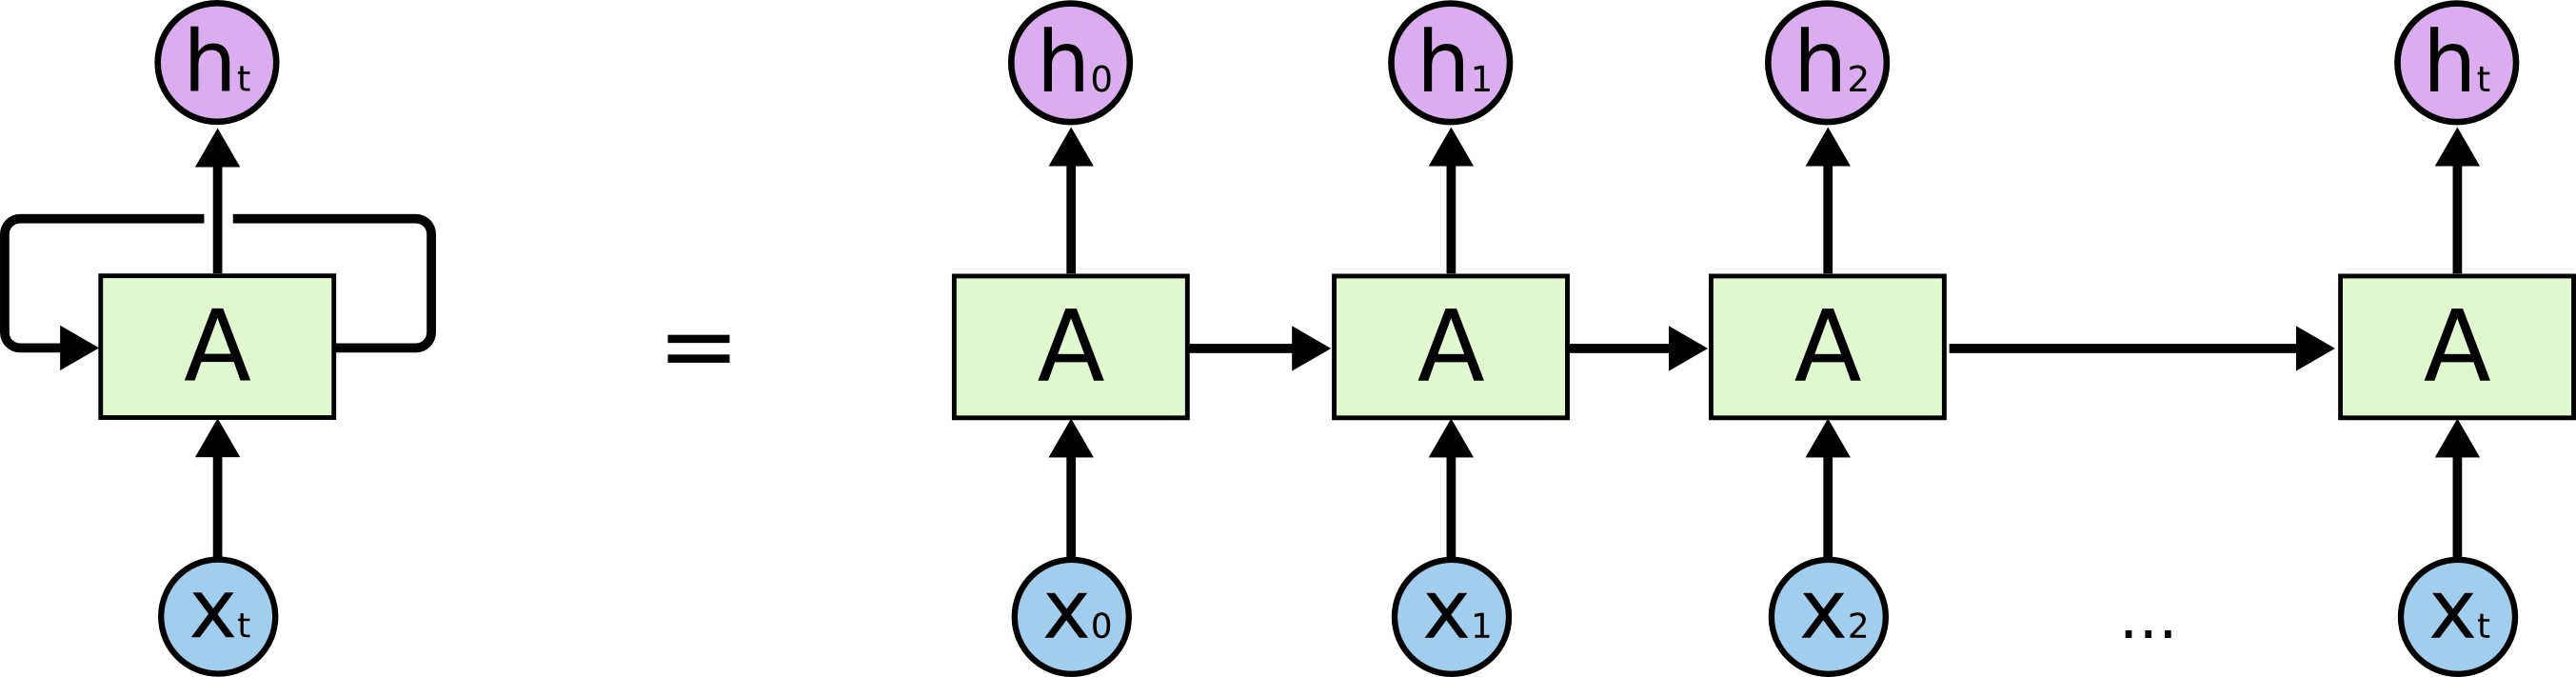
\includegraphics[scale=.22]{RNN-unrolled.png}
        
  }}
  \caption{Unrolled RNN \cite{UnderstandingLSTMNetworks}}
        \label{figurelabel}
     \end{figure}

The notation of symbols in the following is according to elaborations of Jian Guo \cite{guoBackPropagationTime2013}. 
The inputs are denoted by a vector $\mathbf{x}$
with components indexed by $i$. We similarly define the current hidden layer state as vector $\mathbf{s}$ with components indexed 
by $j$, the previous hidden layer state as vector $\mathbf{s}(t-1)$ with components indexed by $h$ and
the output layer as vector $\mathbf{y}$ with components indexed by $k$. 
The weight matrices are written as bold 
uppercase letters where
$\mathbf{V}$ maps $\mathbf{x}$ to the current state $\mathbf{s}(t)$, $\mathbf{U}$ maps the previous hidden 
state $\mathbf{s}(t-1)$
and $\mathbf{W}$ transforms the current state $\mathbf{s}(t)$ to the output layer $\mathbf{y}$. 
For clearness, the previously defined symbols are demonstrated in fig. 2.
Furthermore we describe the relation between outputs and net input function $net_j$ or $net_k$ of a layer 
as the activation functions $f(net_j(t))$ and $g(net_k(t))$ respectively for the hidden and output layer. 
Including biases $b_j$ and $b_k$ for the net input functions, we conclude that the hidden state becomes
(1) and finally the output is described by (3). 

$$
s_j(t) = f(net_j(t)) \eqno{(1)}
$$
$$
net_j(t) = \sum_i^l x_i(t)v_{ji} + \sum_h^ms_h(t-1)u_jh + b_j \eqno{(2)}
$$
$$
y_k(t) = g(net_k(t)) \eqno{(3)}
$$
$$
net_k(t) = \sum_j^m s_j(t)w_{kj} + b_k \eqno{(4)}
$$


\begin{figure}[thpb]
        \centering
        \framebox{\parbox{3in}{
        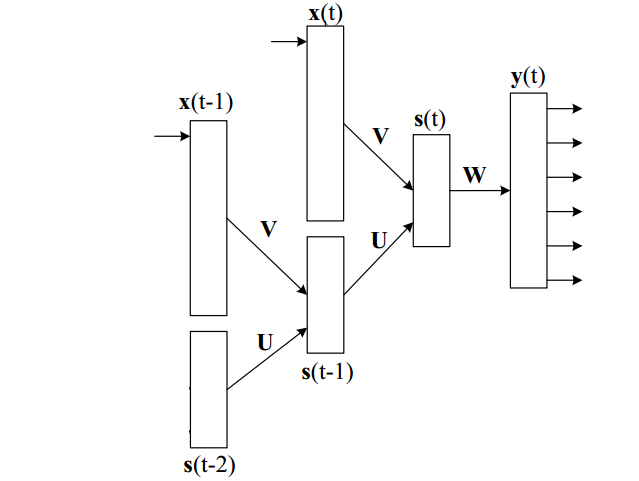
\includegraphics[scale=.3]{rnn_unfolded_guo.png}
  }}
  \caption{An Unrolled RNN with shared weight Matrices $U$ and $V$ between temporal states \cite{guoBackPropagationTime2013} 
  }
        \label{figurelabel}
     \end{figure}


In order to minimize the loss of our network, we define the widely used summed squared error (5) as 
a loss function with desired outputs $d$, total number of training samples $n$ and the number of 
output units $o$. For computational reasons, the stochastic version of gradient descent utilizes 
only subsets of the total training collection, up to the extremum where $p=n$. 
$$
E = \frac{1}{2}\sum_p^n \sum_k^o (d_{pk} - y_{pk})^2 \eqno{(5)}
$$

By propagating this error backwards throughout the network, we can construct the loss function's
derivative with respect to each weight in order to obtain the weight update of a specific weight 
for the next timestep. After application of the chain rule, the weight updates for connections between hidden and output 
layer $\Delta w_{kj}$ result in (6) and for connections between input and hidden layer $\Delta w_{ji}$ 
become (7):

$$
\Delta w_{kj} = \eta \sum_p^n \delta_{pk}s_{pj}=\eta \sum_p^n (d_{pk}-y_{pk})g'(net_{pk})s_{pj} \eqno{(6)}
$$

$$
\Delta w_{ji} = \eta \sum_p^n \delta_{pj}x_{pi}=\eta \sum_p^n\sum_k^o\delta_{pk}w_{kj}f'(net_{pj})x_{pi} \eqno{(7)}
$$

The terms $\delta_{pk}$ and $\delta_{pj}$ are referred to as the components of the specific error vectors 
per layer.
The netfunction of our hidden layer $net_{pj}$ however still depends on the previous state $s_{t-1}$ which in turn 
depends on previous states itself. Unfolding the network up to a temporal depth $\tau$ with the same weights 
throughout the timesteps (fig. 2) allows us to define an error vector for previous time steps as seen in (8).
$$
\delta_{pj}(t-1)= \sum_h^m \delta_{ph}(t)u_{hj}f'(s_{pj}(t-1)) \eqno{(8)}
$$
More detailed reflections on the construction of the equations above can be found in \cite{guoBackPropagationTime2013}.
The procedure previously used to obtain $\delta_{pj}(t-1)$ allows for theoretically arbitrary depths $\tau$
to be recursively calculated. In practice, large values for $\tau$ and the subsequently generated 
long-term dependencies tend to be difficult to handle with gradient descent. This is due to the fact, that
deriving error terms through multiple layers of an unfolded RNN decreases or increases the magnitude of the resulting 
derivative expontially, thus creating phenomena known as vanishing and exploding gradient. 


\subsection{Long Short Term Memory (LSTM)}

These problems occur only when facing long range dependencies in RNNs and can be successfully 
tackled by adopting the Long Short Term Memory Network(LSTM) by Hochreiter and Schmidhuber \cite{hochreiterLongShortTermMemory1997}. 
As shown by Hochreiter, 
a key idea towards avoiding the explosion or vanishing of gradients through a large number of timesteps is 
to enforce a constant errorflow through a single unit $j$ by requiring the net activation derivative of $j$ to follow 
equation 9 with the weight $w_{jj}$ of a single connection to itself.
$$
f'_j(net_j(t))w_{jj}=1.0 \eqno{(9)}
$$
Simple integration over time gives us $f_j(net_j(t))=\frac{net_j}{w_{jj}}$, a linear function. Therefore our recurrent 
definition of $net_j(t+1)=w_{jj}y^j(t)$ leads us to the conclusion, that the unit $j$'s activation has to remain constant (10) 
\cite{hochreiterLongShortTermMemory1997}:
$$
y_j(t+1)=f_j(net(t+1))=f_j(w_{jj}y^j(t))=y^j(t) \eqno{(10)}
$$

This approach alone however leads to a problem that becomes evident during learning in networks with more than one neuron
connected to the so far single unit $j$. The input weights $w_{ji}$ from neuron $i$ and the outgoing weights $w_{kj}$ to neuron $k$ now are 
both responsible for regulating the desired protection from yet unneeded information of previous timesteps as well as conceiving said information
when deemed necessary. Take for instance a language processing network trying to estimate the importance of the subject "You" regarding
the following word sequence "are a tall, friendly, level-headed, smart person". The same weights that have just been trained on this sentence would 
receive conflicting weight updates in the next learning step, when confronted with the new sentence "You are a person". \newline
To overcome this shortcoming, Hochreiter and Schmidhuber propose a more context sensitive approach, using separate gates for forgetting, input and
output regulation within a single cell as seen in fig. 3.   

\begin{figure}[thpb]
        \centering
        \framebox{\parbox{3in}{
        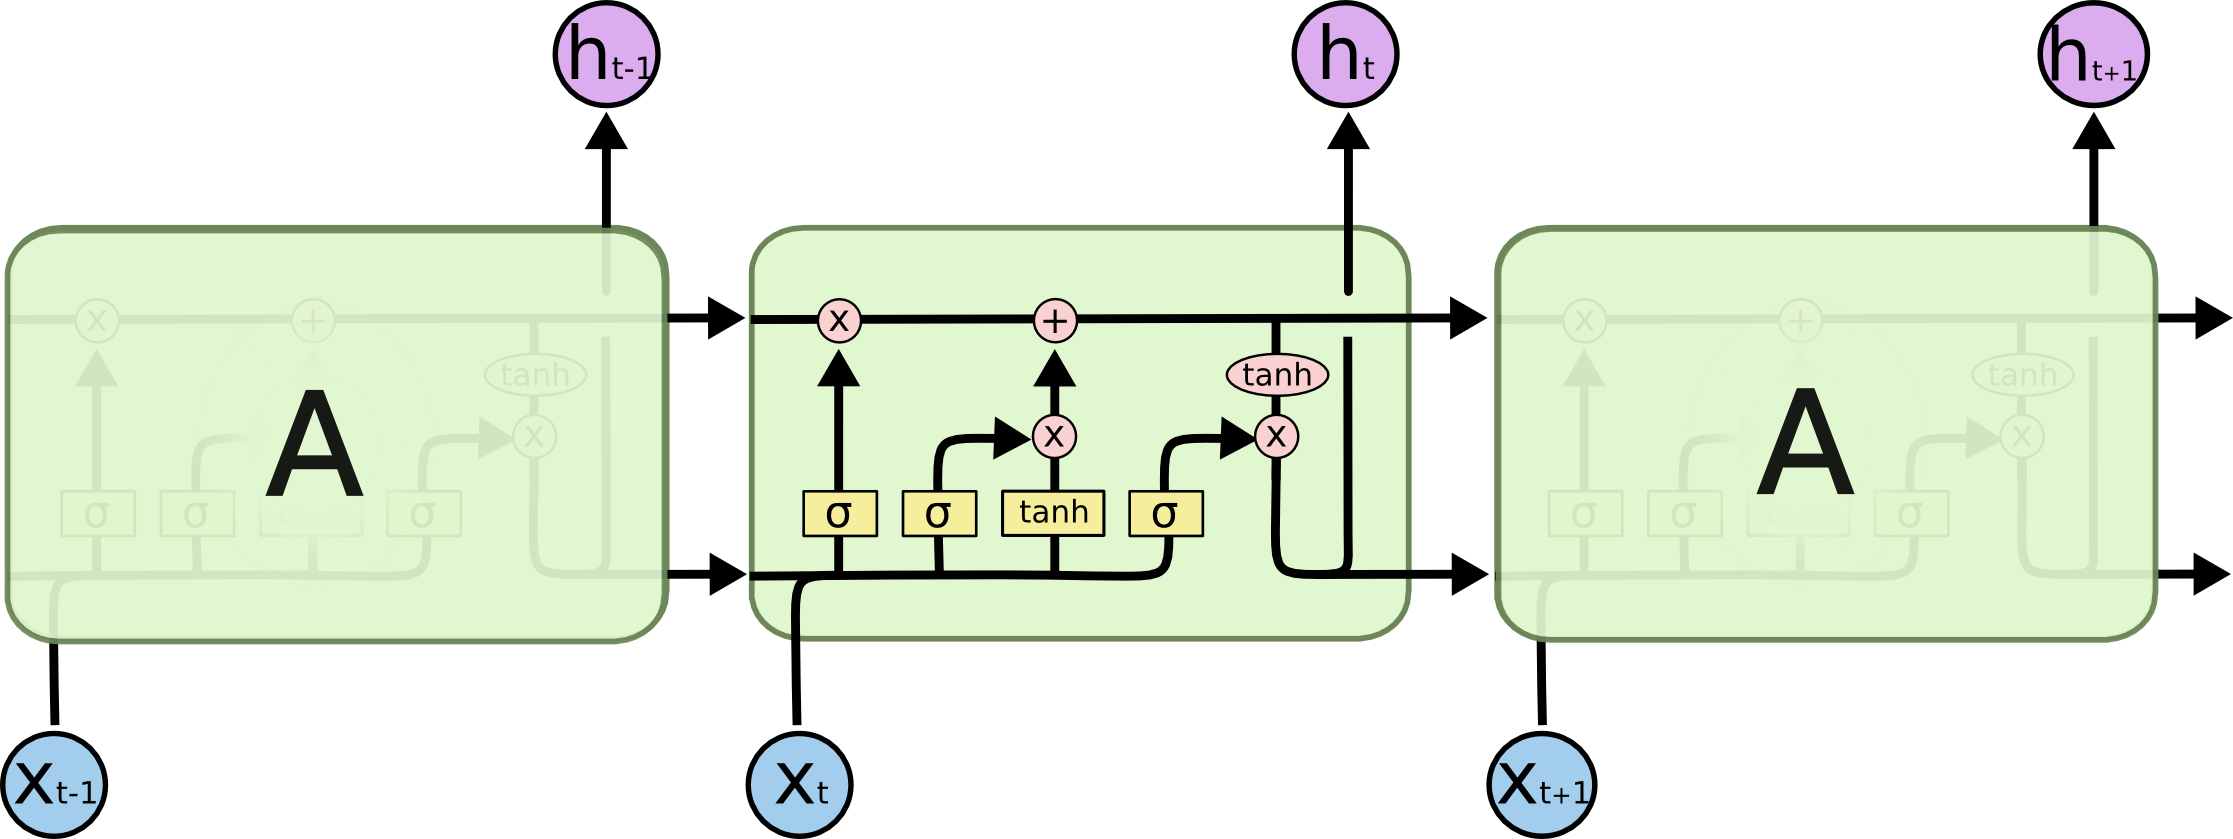
\includegraphics[scale=.265]{LSTM3-chain.png}
  }}
  \caption{Inner composition of an LSTM cell \cite{UnderstandingLSTMNetworks}}
        \label{figurelabel}
     \end{figure}

The $forget\ gate$ consists of a sigmoid-activated layer $f_t$, essentially determining, how much of the previous output $h_{t-1}$ should be kept 
within the LSTM Cell State $C_t$, based on its own set of weights $W_f$ and biases $b_f$:
$$
f_t = \sigma(W_f\times[h_{t-1},x_{t}] + b_f) \eqno{(11)}
$$ 
The $input\ gate$ is composed of the sigmoid-activated layer $i_t$ and the hyperbolic-tangent-activated layer $\tilde{C_t}$, creating candidates
for replacing the current (possibly forgotten) cell state $C_{t-1}$ with $i_t\times\tilde{C_t}$. Each of these layers, again, have their own 
set of weights and biases $W_i$, $b_i$, $W_c$ and $b_c$, leaving us with the respective layer outputs (12) and (13) \cite{UnderstandingLSTMNetworks}:
$$
i_t = \sigma(W_i\times[h_{t-1},x_t]+b_i)  \eqno{(12)}
$$
$$
\tilde{C_t}=tanh(W_c\times[h_{t-1},x_t]+b_c) \eqno{(13)}
$$
In order to determine whether to inhibit possibly disturbing signals to following cell states, the output $h_{t}$ is filtered by applying $tanh(x)$ and 
multiplying with the outcome of the $output\ gate\ layer\ o_t$. The output layer comprises weights $W_o$ and biases $b_o$ and
therefore results in the total output $h_t$:
$$
o_t = \sigma(W_o[h_{t-1}, x_t] + b_o) \eqno{(14)}
$$
$$
h_t = o_t \times tanh(C_t) = o_t\times tanh(f_t\times C_{t-1}+i_t\times\tilde{C_t}) \eqno{(15)}
$$
This design allows for seperate read and write capabilities and therefore enables the capture of error signals within
the cell for longer periods of time than previously possible with standard RNNs \cite{hochreiterLongShortTermMemory1997}. Many applications with
record-breaking performances followed, thus constituting the leading role of LSTMs in temporal problems. Graves and Jaitly 
\cite{gravesEndtoEndSpeechRecognitionwith} provide an   
overview over variations of the vanilla LSTM, such as the introduction of peepholes by Gers and Schmidhuber \cite{gersRecurrentNetsThat2000} 
or the lighter Gated Recurrent Unit (GRU) 
by Cho et al.\cite{choLearningPhraseRepresentations2014}. Furthermore, attention-based models as proposed by 
Graves et al. \cite{gravesNeuralTuringMachines2014}\cite{gravesAdaptiveComputationTime2016} 
and Neelakantan et al.\cite{neelakantanEfficientNonparametricEstimation2015} are promising more recent developments in the field of RNNs.

\section{SPIKING NEURAL NETWORKS (SNN)}

The above described ANN models differ from Feedforward Networks in regards of activation, connection design, learning rules and more, yet implicitly
share a commonground in how they encode information in their neurons. These second generation neural networks, as commonly described in the literature,
activate on continuous functions and make use of their differentiability in backpropagation. Maass et al. \cite{maassNetworksSpikingNeurons1997} 
provide a setup that
integrates a different, biologically more accurate take on modeling neuron activation. These Spiking Neural Networks (SNN) employ
integrate-and-fire neurons \cite{maassNetworksSpikingNeurons} which encode information with an additional temporal factor in its activation pulses, increasing
the density of encoded information.  

\subsection{Neurons - Activation and Signal Processing} 

The fundemantal idea behind the computational units of an SNN builds on integrating a temporal factor 
in the representation of information. Various models of these spiking neurons, such as the integrate-and-fire model
 \cite{abbottLapicqueIntroductionIntegrateandfire1999}, 
the Hodgkin-Huxley model \cite{hodgkinQuantitativeDescriptionMembrane1952}, the model by Izhikevich \cite{izhikevichSimpleModelSpiking2003}
and the Spike Response Model by Gerstner \cite{gerstnerSpikeresponseModel2008}
exist and vary in their attempt to trade off biological accuracy and computational complexity \cite{gruningSpikingNeuralNetworks2014}.
The Leaky-Integrate-and-Fire model is arguably the most widespread apporach due to its simplicity and computational advantages. 
The representation of the activation process of the neron is modeled by an electrical circuit in which the membrane potential, threshold voltage,
resting potential and leak rate are realized through a capacitor, gate, battery and resistance
\cite{abbottLapicqueIntroductionIntegrateandfire1999}\cite{ponulakIntroductionSpikingNeural2011}.
\subsection{Spike-based Neural Codes}

Whilst encoding and decoding of the desired information is rather straight forward in second generation neural network models,
this challenge proves harder for the time-dependent neurons in an SNN, due to the arbitrary 
number of theorically possible ways of encoding information in the neurons. In fact, the biological process of information decoding is 
still being researched, whereas various methods have been discussed in Neuroscience and Machine Learning:

\begin{itemize}

        \item Rate Coding is an approach aiming at recording spike rates during fixed time frames. 
        This implementation of spike encoding can be seen as an analog way of interpreting spike trains in SNNs.
        \item Latency Coding encodes spikes based on their timing rather than their multiplicity. This encoding 
        has for example been used in unsupervised learning, and
        supervised learning methods like SpikeProp \cite{bohteSpikePropBackpropagationNetworks}
        \item Fully temporal codes are a more general term which includes the above mentioned approaches. It encodes information based on the precise
        timing of each spike in a spike train\cite{gruningSpikingNeuralNetworks2014}
        \item Gaussian Coding applies a gaussian distribution over recorded spikes of each 
        neuron and encodes information based on their stochastic occurence.
\end{itemize}        

\subsection{Learning in Spiking Neural Networks - Synaptic Plasiticity}

While conventional neural networks employ a stochastic version of gradient descend to backpropagate erros throughout the network, the same approach
is difficult to apply in the realm of SNNs due to their temporal dependancies and the non-differentiability of spike trains. Whereas multiple learning
rules adressing SNNs exist (such as Hebbian Rule, Binarization of ANNs, Conversion from ANNs and Variations of backpropagation 
\cite{pfeifferDeepLearningSpiking2018}), 
a state-of-the-art algorithm such as backpropagation has yet to emerge. We will first focus on a more 
biologically motivated training rule called spike-timing-dependant plasiticy (STDP). The key feature of this approach is 
to adjust weights between a pre- and post-synaptic neuron according to their relative spike times within an interval of roughly tens of 
milliseconds in length \cite{bohteSpikePropBackpropagationNetworks}. If a postynaptic neuron fires shortly after its presynaptic neuron, the connecting weights is strengthended
whereas presynaptic neurons firing after the postsynaptic neuron will lead to weakening of the weights. The experimentally refined and 
commonly used formula according to dan et al. \cite{danSpikeTimingdependentPlasticity2006} for the exact weight updates is given in (16)
$$
\Delta w = \left\{
        \begin{array}{ll}
            Ae^{\frac{-(|t_{pre}-t_{post}|)}{r}} & \quad t_{pre}-t{post}\leq 0, A>0 \\
            Be^{\frac{-(|t_{pre}-t_{post}|)}{r}} & \quad t_{pre}-t{post}>0, B<0
        \end{array} 
    \right. 
    \eqno{(16)}
$$ 

where $\delta w$ is the update of the weight $w$ with adjustable learning rates $A$, $B$ and pre/postsynaptic fire times $t_{pre}$/$t_{post}$. A 
related rule to STDP is the more general hebbian learning rule, which in contrast to STDP claims, that synaptic efficiacy arises from the 
general temporal proximity of these signals independant from the order of occurence. This rule is often referred to as "fire-together-wire-together".
Both mentioned approaches are illustrated in fig. 4.

\begin{figure}[thpb]
        \centering
        \framebox{\parbox{3in}{
        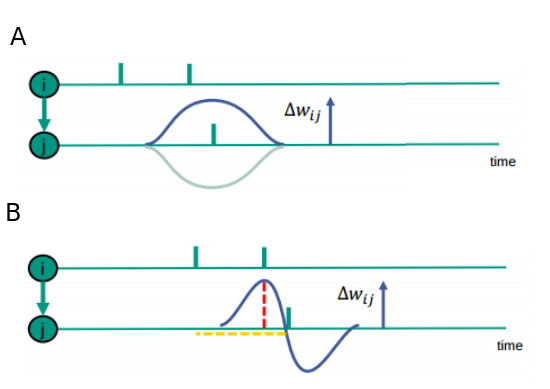
\includegraphics[scale=.4]{stdp_hebbian2.png}
  }}
  \caption{\textbf{A: } illustration of weight-updates $\Delta w_{ij}$ with presynaptic neuron $i$ and postsynaptic neuron $j$ according to STDP \newline 
  \textbf{B: } symmetric hebbian learning rule with weight update $\Delta w_{ij}$, presynaptic neuron $i$ and postsynaptic neuron $j$}
        \label{figurelabel}
\end{figure}

The above mentioned learning rules share the common characteristic in which they don't require information other than what is available 
in a local neighborhood of neurons. Therefore they do not require the biologically unrealistic 
transport of weight information throughout numerous layers of neurons \cite{samadiDeepLearningDynamic2017} \cite{chintaAdaptiveOptimalControl2012}
\cite{crickRecentExcitementNeural1989}\cite{decoNeurodynamicalCorticalModel2004}. Consequently, these learning rules 
are suited for unsupervised learning tasks and pose interesting 
insights from a neuroscientific standpoint. Guyonneau et al. \cite{masquelierSpikeTimingDependent2008} \cite{tavanaeiDeepLearningSpiking2019}
showed, that STDP-equipped SNNs are capable of learning input 
patterns and decrease latencies between in- and output throughout training. Furthermore, T. Masquelier \cite{masquelierSpikeTimingDependent2008}
and S. R. Kheradpisheh \cite{tavanaeiDeepLearningSpiking2019} point out, that 
the increased density of encoded information in SNNs allows even a single neuron to learn spatio-temporal patterns. However practical usability
of these learning rules raises the need for proper supervised learning algorithms, often clashing with mathematical feasibility, numerical efficiency 
or biological plausibility. In this, we encouter problems, such as the non differntiability of spikes and the biological abscence of outer error 
signals in deeper layers. These challenges remain generally unsolved, however various promising advances have been proposed in tackling them.
In a rather biological aspect, Markov et al.\cite{markovAnatomyHierarchyFeedforward2014} propose the existance of
feedback connections, designed to project information within
hierarchically organized networks. Approaches such as SpikeProp by Bohte and Kok deal with discontinous nature of spiking neurons by linearizing 
the relationship between post-synaptic input and the resulting spiking time, consequently circumventing the discontinuity of the 
thresholding function \cite{bohteSpikePropBackpropagationNetworks}. Further techniques aiming at surrogating the gradient of 
discontinuous activations have been researched 
and implemented by Neftci et al. \cite{neftciSurrogateGradientLearning2019}.


\subsection{Eligibility Traces}
When performing on tasks that last between few seconds to multiple minutes until an output of an ANN can be evaluated, it can be 
difficult to assign blame or reward for the achieved outcome to particular spikes which usually happen within the range of few milliseconds. 
Accordingly, the field of Reinforcement Learning and Neuroscience provide an approach to close this temporal gap by introducing 
a dynamic variable in synapses henceforth called eligibility trace \cite{seungLearningSpikingNeural2003}. Eligibility traces 
record recent synaptic activity and enable better
assignment of error signals to culprit neurons. Neuroscience suggests, that eligibility traces may be a key feature to 
neuromodulatory reward based learning such as the midbrain dopaminergic system \cite{panDopamineCellsRespond2005}. Updates to the 
eligiblity trace are described
by the eligibility function $f_c(t)$ in close accordance to STDP spike patterns of pre-/postsynaptic and post-/presynaptic spike pairs. Respectively, 
a pair of spikes will increase or decrease the eligibility trace $c_{ji}(t)$ of the synpase over time (fig. 5 A). Reward signals $d(t)$ 
received after a time delay can now be assigned to synapses using a learning rule that changes synaptic weights proportionally to the product of
$c_{ji}(t)$ and $d(t)$, (17).

$$
\frac{d}{dt}w{ji}(t) = c_{ji}(t)d(t) \eqno{(17)}
$$ 

\begin{figure}[thpb]
        \centering
        \framebox{\parbox{3in}{
        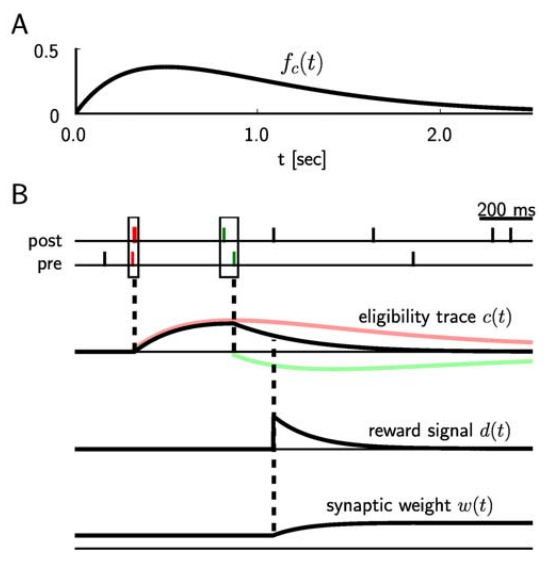
\includegraphics[scale=.35]{etraces.png}
  }}
  \caption{\textbf{A:} Eligibility function fc(t). Illustrated are values for a pre-/postsynaptic spike pattern. Negative for
  post-/presynaptic spike patterns. \newline
  \textbf{B:} Contributions of spike patterns (red and green) to an eligibility trace $c(T)$ and the according
  weight update $w(t)$ upon reception of a reward $d(t)$.\cite{legensteinLearningTheoryRewardModulated2008} }
        \label{figurelabel}
     \end{figure}

\section{LEARNING TO LEARN (L2L)}

The field of reinforcement learning (RL) has recently celebrated great success at reaching human-like and even surpassing human abilities on
complex environments such as Atari \cite{mnihAsynchronousMethodsDeep2016} and Go \cite{silverMasteringGameGo2016} with the implementation 
of Deep Neural Networks to 
account for non-linear function approximation over high-dimensional action and state spaces. However Artificial Intelligence in general 
\cite{lansdellLearningtolearn2018} and Reinforcement Learning in particular \cite{duanRLFastReinforcement2016} currently
suffer from two major drawbacks, 
that are limiting their application and design \cite{wangLearningReinforcementLearn2016}:
\begin{itemize}
        \item Firstly the immense volume of required training data and the relatively expensive generation of this data in often simulated
        environments.
        \item Secondly RL-algorithms often have to be heavily tailored to a specific range of tasks and various algorithms, each of which
        depending on numerous hyperparameters and thus requiring immense computational efforts.
\end{itemize}        

Botvinick et al. \cite{botvinickReinforcementLearningFast2019} explain these weak spots in AI with a need for low 
learning rates and the bias-variance trade-off.
Low learning rates are necessary to prevent both catastrophic interference (discarding previously reached successful
configurations) and overfitting \cite{hardtTrainFasterGeneralize2015}. The bias-variance trade-off is describes the contrary 
working directions of efficiency-driving biases or priors and performing on a wider range of tasks. \newline

Learning to Learn (L2L) addresses these issues, by mimicking human learning behaviour to extract abstract information on wide
families of tasks, thus reducing the required training data for any more specific subtask. Landsell and
Kording\cite{lansdellLearningtolearn2018} argue, 
that these L2L approaches can be categorized into 
either Learning to Optimize or Structure Learning. Learning to Optimize focusses on the general 
adaption of network parameters to achieve efficient learning rules on arbirary Task classes without hand-selection. Similiarly to the way
gradient descent applies small changes of the weights in an NN in order to minimize loss functions, the design of AI systems can be viewed as
an optimization problem itself, that requires parameter optimization to ensure a well performing algorithm. Structure Learning 
on the other hand makes use of structural similarities within a finite family of tasks to reach higher data
efficiency due to its prior adaptnedness to the given family of tasks \cite{lansdellLearningtolearn2018}. \newline

\begin{figure}[thpb]
        \centering
        \framebox{\parbox{3in}{
        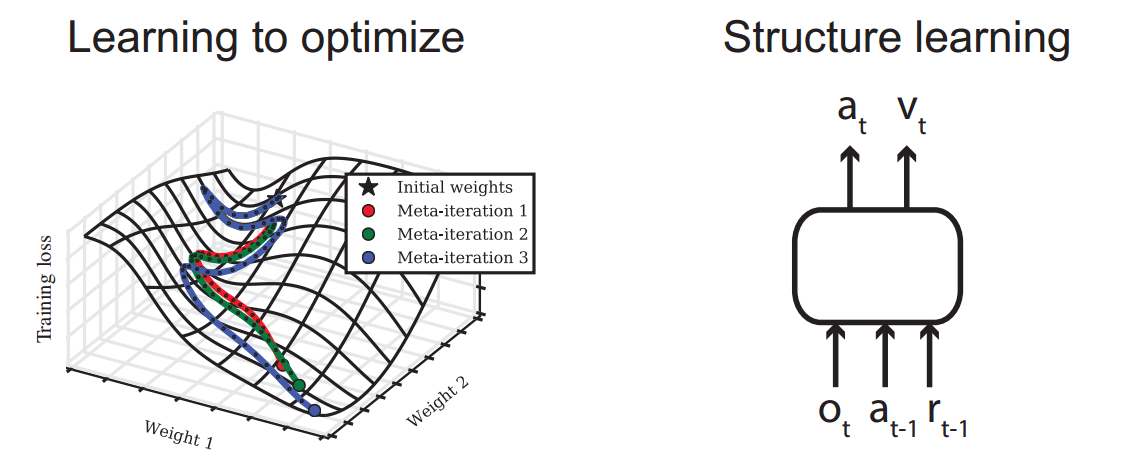
\includegraphics[scale=.19]{L2Optimize_StrLearning_Landsell.png}
  }}
  \caption{Types of learning-to-learn in AI. Learning-to-learn can be roughly divided into learning to optimize and structure learning.
  In AI, hyperparameter optimization is
  an example of learning to optimize \cite{maclaurinGradientbasedHyperparameterOptimization}, while a 
  recurrent neural network taking rewards, actions and observations
   can often be used to perform structure learning \cite{wangLearningReinforcementLearn2016} \cite{lansdellLearningtolearn2018}.}
        \label{figurelabel}
     \end{figure}


\subsection{Learning to Reinforcement Learn (metal-RL) and RL²}

A high level architecture consisting of a learner (performing on the task itself) and a meta-learner (adjusting the learner) is
inherent to most implementations of L2L \cite{lansdellLearningtolearn2018} and has been refined in various ways to create new L2L Systems, as will be
explained in the following section.

Wang et al.\cite{wangLearningReinforcementLearn2016} as well as Duan et al.\cite{duanRLFastReinforcement2016} introduced 
frameworks that can be thought of as generating an RL algorithm of their own and
provide agents, who are given a predesigned prior to efficiently learn any task $T \epsilon F$ (in the original papers denoted as 
a Markov Decision Process (MDP) $m \epsilon M$) from a family of interrelated fasks $F$(i.e. a set of MDPs $M$). 

In their attempt to design an algorithm, capable of performing well on a set $M$ of Markov Decision Processes (MDPs), Duan et al. implement a nested
system in which learning an RL algorithm is regarded as a reinforcement learning problem itself, hence the name RL² 
\cite{duanRLFastReinforcement2016}. The agent performing 
on a randomly drawn separate MDP $m \epsilon M$ from the distribution $\rho_{M} : M \longrightarrow R_{+}$ is represented as an RNN
which outputs the probability distribution over the tasks action-space $\pi$ (policy) based on a function $\phi (s,a,r,d)$ of 
the tuple (state, action, reward, termination flag) (Duan et al.). On a higher abstraction layer, this RNN is being 
optimized by an implementaion of Trust Region Policy Optimization (TRPO), a 
state-of-the-art DRL algorithm \cite{schulmanTrustRegionPolicy2015} with several advantages regarding stability
 and hyperparameter dependance.\newline

\begin{figure}[thpb]
        \centering
        \framebox{\parbox{3in}{
        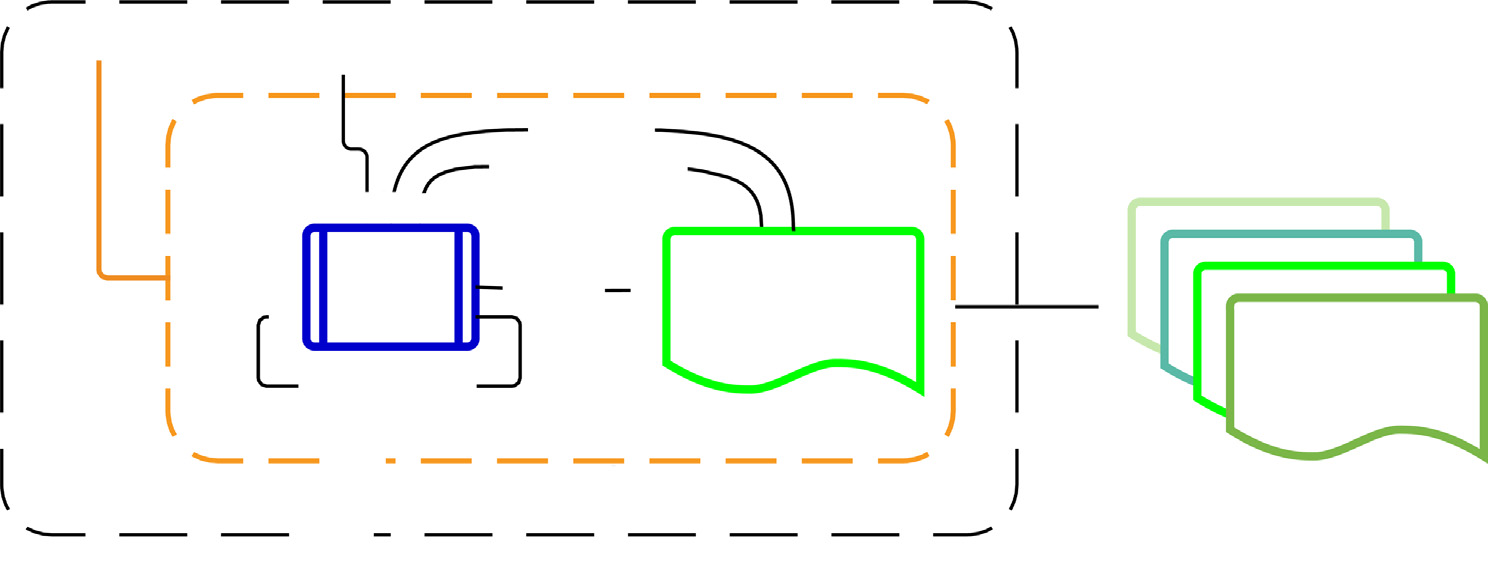
\includegraphics[scale=.24]{meta-RL_Botvinick.png}
  }}
  \caption{Schematic of Meta-reinforcement Learning, Illustrating the Inner and Outer Loops of Training. The
  outer loop trains the parameter weights $\theta$, which determine the inner-loop learner (’Agent’, instantiated by a recurrent
  neural network) that interacts with an environment for the duration of the episode. For every cycle of the outer loop, a new
  environment is sampled from a distribution of environments, which share some common structure \cite{botvinickReinforcementLearningFast2019}.}
        \label{figurelabel}
     \end{figure}

Wang et al.\cite{wangLearningReinforcementLearn2016} define a similiar setup in which a RL-algorithm is responsible for 
learning the weights of a nested RNN. Both, inner and outer loop 
in this framework draw their learning experience from the reward information generated by the actions of the RNN, where 
the RNN holds information on the previously chosen action and the subsequent rewards. However the process of learning
in each of these loops is realized differently and results in specializations of different scopes. While the wrapping RL-algorithm used to 
optimize the weights of the RNN operates over the entire set of episodes, that is to say all MDPs $M$, learning of the nested RNN 
within a single task $m$ is based on the inner recurrent dynamics of the network. Notably, the RNN 
is able to encode learned experience on a specific task using only its inner memory variables, leaving us with the observation
that a well working short-term memory is a key factor to learning on different levels of abstraction. 
The policy outputs $\pi$ of this network can then
be viewed as an RL-algorithm on its own, resulting in the name meta-RL. For the implementation of this framework Wang et al.
\cite{wangLearningReinforcementLearn2016} 
used an LSTM according to Hochreiter and Schmidhuber \cite{hochreiterLongShortTermMemory1997} to account for the inner RNN, while both synchronous 
asynchronous advantage actor critics (A2C and A3C) (Mnih et al.) were employed to learn inter-cell weights.
The observation vectors of experiment environments
were either directly fed to the LSTM one-hot-encoded or passed through an additional deep encoder model\cite{wangLearningReinforcementLearn2016}. 
Experiments on a series of bandit problem and two
MDP-centered problems with implementation architectures as described above showed, that meta-RL delivers 
competitive results compared to problem-specific algorithms (Thompson sampling, UCB, Gittins) while operating on a 
wider set of tasks. \newline

\begin{figure}[thpb]
        \centering
        \framebox{\parbox{3in}{
        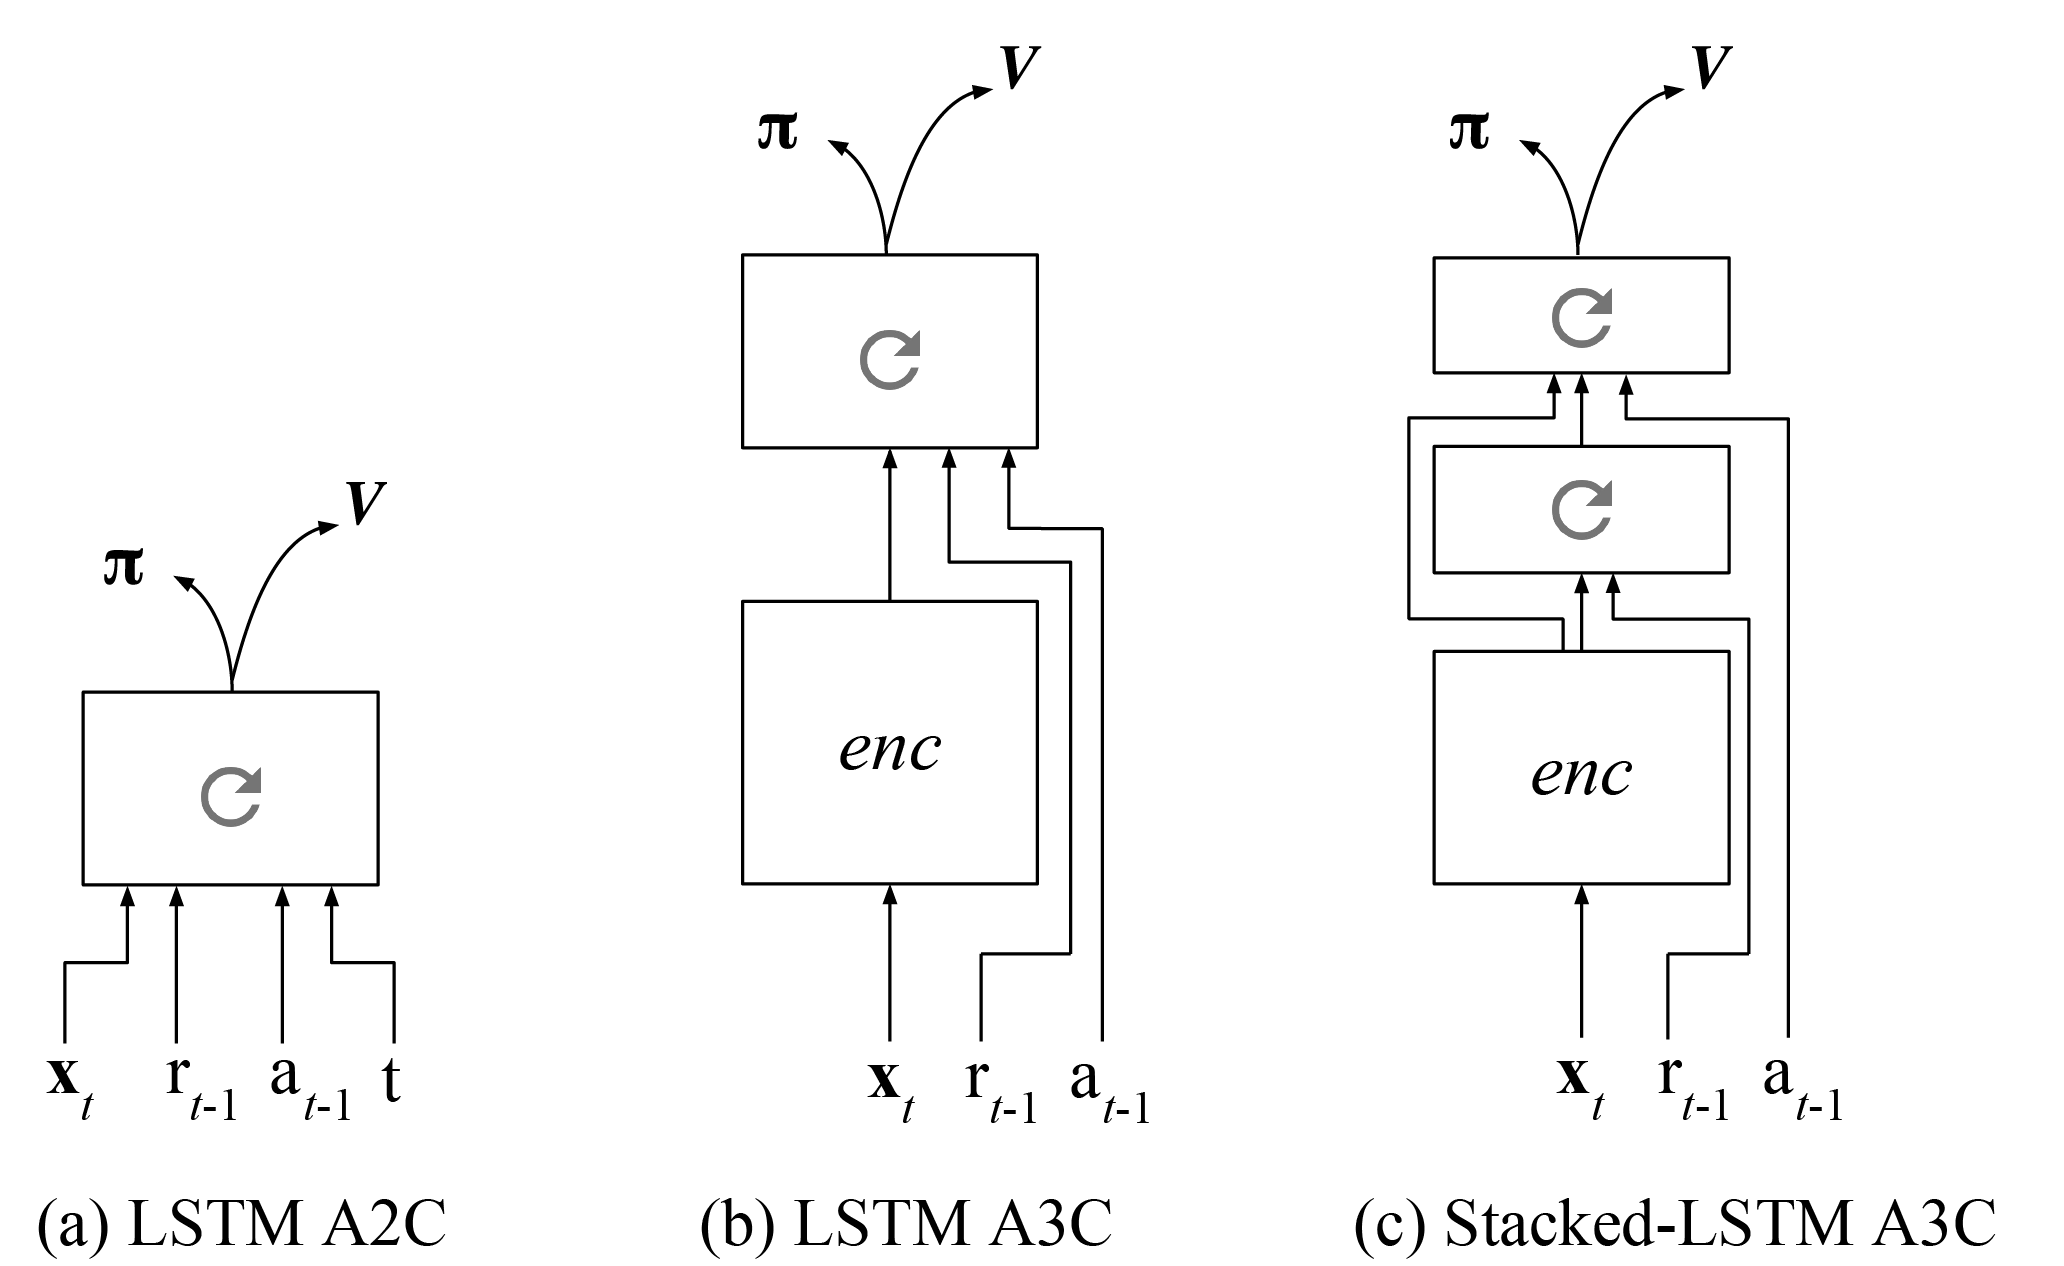
\includegraphics[scale=.29]{metaRL_arcs_Wang.png}
  }}
  \caption{\textbf{b:} Convolutional-LSTM architecture with autoencoder and A3C \newline
        \textbf{c:} Stacked-LSTM architecture with additional recurrent network. Rewards and actions are given to different stack 
        RNNs \cite{wangLearningReinforcementLearn2016}}
        \label{figurelabel}
     \end{figure}
  

A notable characteristic of both previously described setups is that the learning rate of the nested RNN is chosen lower compared 
to the outer optimization loop, consequently preventing
the agent from overfitting to a single task $m$, yet gathering knowledge from the entire MDP space $M$ 
\cite{botvinickReinforcementLearningFast2019}.\newline


\subsection{L2L in the Context of Spiking Neural Networks}
When applied to Networks of Spiking Neurons, the previously described framework of L2L offers a promising alternative
to common approaches which embed a series of biologically implausible ingredients. One major biological implausibility
in learning algorithms employing error feedback is suggested by evidence, that real neurons almost certainly lack weight transport
when unrolling the chain rule of backpropagation on the backward pass\cite{samadiDeepLearningDynamic2017}
\cite{chintaAdaptiveOptimalControl2012}\cite{crickRecentExcitementNeural1989}. In order 
to calculate gradients
of an error at the outputs of a network, these neurons would have to maintain information about the strenth of synapses outside their local
neighborhood, which seems unrealistic from a biological point of view. This evidence suggests the existence of a more sophisticated 
system of learning signals, which dont require information on global synaptic weights. Furthermore, oversimplistic models of real
neurons, such as the Leaky integrate-and-fire neuron, lack key characteristics of real neurons and are often even further modified by engaging
derivative surrogate functions in order to deal with the non-differentiable nature of spiking neurons. Among these mismatches between 
biological neurons and their artifical models is the ability of biological neurons, to adapt to previously experienced inputs
and weights \cite{samadiDeepLearningDynamic2017}. The ability to adapt to previous spikes of presynaptic neurons however not merely represents a visual
difference but can be interpreted as the ability to store temporal information. \newline
By deploying adaptive LIF neurons in a Network of Spiking Neurons, Bellec et al.\cite{bellecLongShorttermMemory2018} were able to overcome not only a 
discrepancy between model and reality but also achieved a well working long short-term memory, thus creating a new type of RNNs, the LSNN. 
Here, the adaptivity of neurons is realized by increasing the firing threshold $B_j(t)$ of a neuron $j$
by a fixed amount $\frac{\beta}{\tau_{a,j}}$ for incoming spike trains $z_j(t)$ and decaying it exponentially to a baseline $b^0_j$ value in spike-free intervals 
with time constant $\tau_{a,j}$. The time constant can be chosen to fit the desired range of the created short-term memory. For discrete timesteps
of $\delta t = 1 ms$ the dynamics of the adaptive threshold becomes (18) with the recursive update rule (19):
$$
B_j(t) = b^0_j + \beta b_j(t) \eqno{(18)}
$$
$$
b_j(t+\delta t) = e^{-\frac{\delta t}{\tau_{a,j}}} b_j(t)+(1-e^{-\frac{\delta t}{\tau_{a,j}}})z_j(t) \eqno{(19)}
$$
As pointed out in the meta-RL, a well-working short-term memory is crucial to the ability to store learned experience on different levels
of abstraction and now allows for the application of L2L to a network of spiking neurons. On a side note, the increase of the firing 
threshold in the adaptive neurons clearly leads to an overall decrease of spikes, thus operating more energy efficiently when deployed 
on neuromorphic hardware.  
The network  architecture comprises additional sets of non-adaptive excitatory and inhibitory LIF neurons
\cite{bellecLongShorttermMemory2018}(fig. 9). Similarly to 
Wang et al.\cite{wangLearningReinforcementLearn2016}, 
the synaptic weights of this network are subject to optimization of an outer loop algorithm, in this case a combination of
BPTT and a biologically inspired rewiring method called DEEP R \cite{bellecDeepRewiringTraining2017}(fig. 9). Since BPTT requires 
calculation of error gradients, the authors utilized a pseudo-derrivate to surrogate the non-existing derivative of neuronal spike trains 
with a simple damped triangular function. The synaptic weights are updated only after completed runs of tasks, while in-task 
optimzation is realized through internal memory dynamics according to (17) and (18). Further details on the network setup and implementation 
can be reviewed in \cite{bellecLongShorttermMemory2018}.
\newline
\begin{figure}[thpb]
        \centering
        \framebox{\parbox{3in}{
        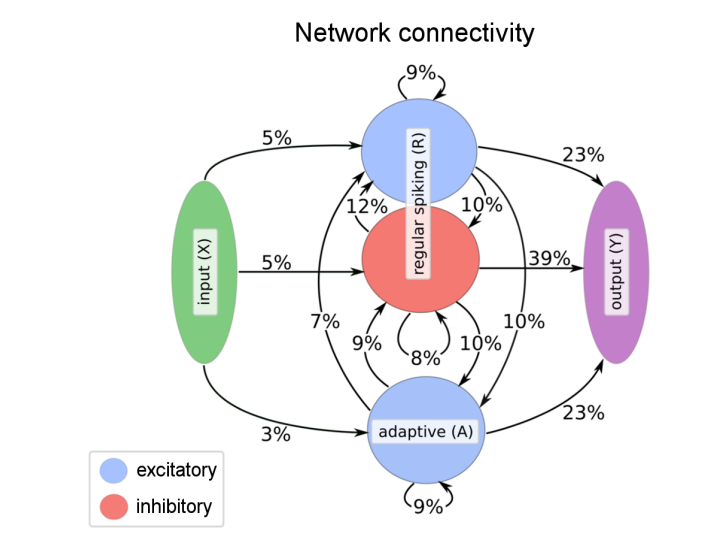
\includegraphics[scale=.28]{lsnn.png}
}}
\caption{Basic architecture of LSNN. Percentages on sypatic connections represent connectivity of the LSNN after applying DEEP R 
in conjunction with BPTT. 
Populations X,Y and R of regular spiking LIF neurons coupled with 
a population A of adaptive LIF neurons. \cite{bellecLongShorttermMemory2018}}
        \label{figurelabel}
        \end{figure}

The results of this model might already offer interesting perspectives from a biological and neuroscientific view, however one 
is tempted to wonder if
this framework can be applied to more biologically plausible models. Recall that the previously described setup including BPTT
still requires the transport of global weight information as well as a transmission of error signals through time which are 
widely considered implausible in real RNNs. Bellec et al.\cite{bellecBiologicallyInspiredAlternatives2019} consequently 
developed an approach designed to tackle these shortcomings. The chapter $eligibility\ traces$ already hinted at the possibility of 
avoiding the need
for weight transport in credit assigment by conducting error propagation through dynamic eligibility traces. Bellec et al. take up
the learning rule (17) with a different motiviation, namely the approximation of error gradients. The fundamental role of eligibility traces  
in this algorithm led to the name e-Prop. The underlying basis for e-Prop is the assumption, that error gradients w.r.t. a synaptic 
weight $\theta_{ji}$ can be factorized into a learning 
signal $L^t_j$ and its eligibility trace $e^t_{ji}$, summed up over time\cite{bellecBiologicallyInspiredAlternatives2019}:

$$
\frac{dE}{d\theta_{ji}} = \sum_t L^t_j e^t_{ji} \eqno{(20)}
$$

Bellec et al.'s claim for biological plausibility is coupled to obtaining the learning signal $L^t_j$ in a way, that does not require 
a propagation of error gradients through time or numerous layers (fig. 10). In the following we will focus on two different approximizations
for these learning signals $\hat{L}^t_{j1}$ and  $\hat{L}^t_{j2}$ constituting two versions e-Prop 1 and e-Prop 2. \newline
\begin{figure}[thpb]
        \centering
        \framebox{\parbox{3in}{
        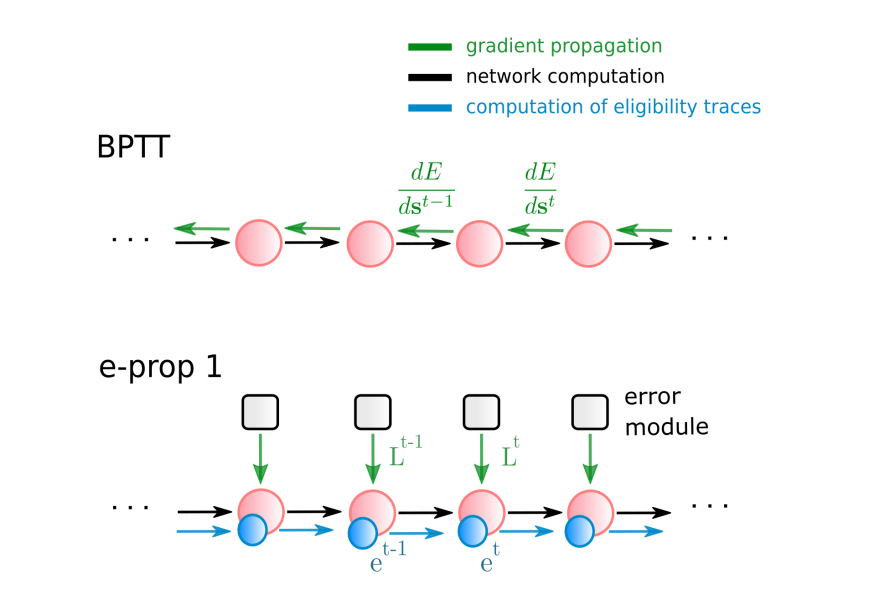
\includegraphics[scale=.26]{eprop1pass.png}
  }}
  \caption{Illustration of the error signal flow throgh network layers. Evidently, e-prop 1 does not require information transport
  in a backwards pass. (edited from \cite{bellecBiologicallyInspiredAlternatives2019})
  }
        \label{figurelabel}
     \end{figure}

E-Prop 1 uses the findings described in $feedback\ alignment$ to braodcast error signals directly to the affected synaptic weights 
while adopting a random weight matrix instead of the actual weights. Assuming an error at the output layer $k$ of leaky readout neurons 
$y^t_k$ of $((y^{*,t}_k-y^t_k)$ our Learning signal to a neuron $\theta ^{rec}_{ji}$ thus becomes $\sum_k B^{random}_{jk}(y^{*,t}_k-y^t_k)$
instead of $\sum_k \theta^{out}_{kj}(y^{*,t}_k-y^t_k)$. Since this network is an RSNN, these learning signals are broadcasted to all synaptic
weights in different time slices of an unrolled recurrent network. The authors however reached better results when choosing the random 
weight projection matrix to be constant over all time-slices.

\begin{figure}[thpb]
        \centering
        \framebox{\parbox{3in}{
        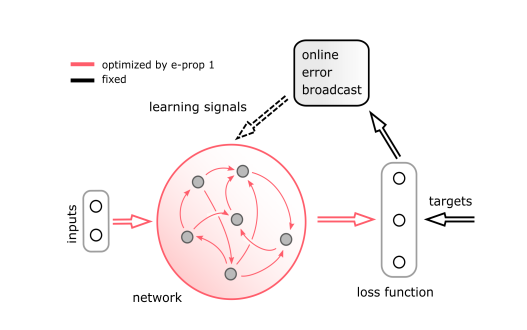
\includegraphics[scale=.4]{eprop1.png}
  }}
  \caption{Basic architecture of e-prop 1. Error broadcasts are calculated online at the output layer and sent directly
  to deeper layers of the RSNN, avoiding the necessity for weight transport on the backwards pass.(edited 
  from \cite{bellecBiologicallyInspiredAlternatives2019})
  }
        \label{figurelabel}
     \end{figure}
     
This approach is applicable to architectures with short-term memory, such as LSNNs, thus providing a basis for L2L frameworks, where 
learning on different levels could be allocated to the outer optimization through e-prop 1 and inner adaptive memory variables. 
\newline
However Bellec et al. developed a second version of e-Prop, specifically dedicated to the utilization of L2L, called e-Prop 2. 
Neuroscience has long considered the existence of a sophisticated system of error feedback generation, where a sudden sharp 
negative potential in the brain called error-related negativity (ERN) is suspected to play a role in reflecting such error signals.
ERN accompanies motoric misbehaviour responses and typically peaks within 80ms - 120ms after beginning of an error signal 
\cite{gehringErrorRelatedNegativity2018}\cite{dikmanErrorMonitoringReward2000}.
However further research remarkably points out that ERN can be observed even before motoric feedback becomes evident through 
sensory feedback, implying the existence of additional error response- and prediction systems embedded in biological neural networks
\cite{macleanUsingBrainPotentials2015}
which may well be a result of evolutionary development.
Motivated by this finding, Bellec et al.\cite{bellecBiologicallyInspiredAlternatives2019} engaged an additional 
RSNN solely designed to generate optimized learning signals in e-Prop 2's architecture.
These error-modules now take over the role of an outer-loop meta learner as mentioned in the chapter "meta-RL". Learning of the error module 
is again accomplished by training on a whole family of tasks $F$ with BPTT. Conceivably, the application of BPTT contradicts the claim for 
biological plausibility, howbeit the authors argue that the origin of 
well-developed systems of error-prediction and signal-generation are not fully understoof but do not require biologically plausible optimization 
algorithms if interpreted as priors formed by a long process of evolution. The error module contains weights $\Psi$ and receives the  
inputs $\mathbf{x^t}$ and a target vector $\mathbf{y^{*,t}}$ which may be the target output of the network or a desired target state 
(e.g. a target vector may 
be the position of a robotic manipulator at time $t$, while the network output are joint velocities) \cite{bellecBiologicallyInspiredAlternatives2019}.
A distinct difference 
between this setup and meta-RL or L2L LSNNs lies within the split network neurons of outer meta-learner and inner learner. Since the outer error
modules now posess their own set of neurons with weights $\mathbf{\Psi}$, the inner learner can store learned experience in 
its own set of synaptic weights
$\mathbf{\theta}$, implicitly alleviating the categorical need for short-term memory. \newline

\begin{figure}[thpb]
        \centering
        \framebox{\parbox{3in}{
        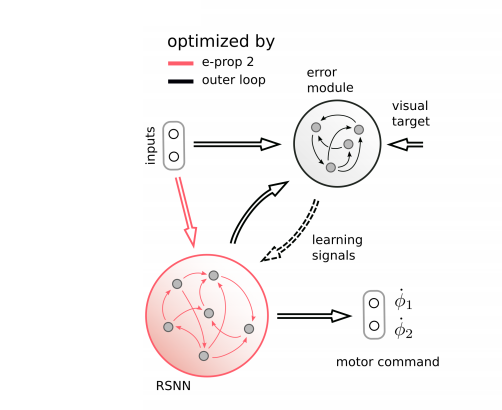
\includegraphics[scale=.4]{eprop2.png}
  }}
  \caption{ Basic architecture of e-prop 2. An Error module network receives network inputs, a target state and the network state to 
  produce learning signals optimized to improve learning in a nested RSNN (edited from \cite{bellecBiologicallyInspiredAlternatives2019}).
  }
        \label{figurelabel}
     \end{figure}

Training of this model is split into a training phase and a testing phase both consisting of exactly one trial. The initial output of the 
inner learner considering a specific task $C$ therefore depends on its initial set of weights $\mathbf{\theta_{init}}$. 
As e-Prop 2 optimizes $\mathbf{\theta_{init}}$
after a single training trial using its own initial weights $\mathbf{\Psi_{init}}$, the output on the test trial with the same specific task $C$ is 
now a result of the improved priors $\mathbf{\theta_{test,C}}$. A cost function for BPTT in the error module is created from the results of the test run
$L_C(\mathbf{\theta_{test,C}})$. The complete learning dynamics of e-Prop 2 are then described by the minimization problem (21) and the 
update rule (22):
$$
min\{ \mathbf{E}_{C\forall C\epsilon F}[L_C(\mathbf{\theta_{test,C}})]\} \eqno{(21)}
$$
$$
(\mathbf{\theta_{test,C}})_{ji} = (\mathbf{\theta_{init}})_{ji} - \eta \sum_t \hat{L}^t_j e^t_{ji} \eqno{(22)}
$$

Duan et al.\cite{duanOneShotImitationLearning2017} identified the outer-loop optimization algorithm as an imminent 
bottleneck to this approach, hence it comes as 
little surprise, that further approaches such as the work by Bohnstingl et al.\cite{bohnstinglNeuromorphicHardwareLearns2019}
 have aimed at designing better outer-loop algorithms.
The unsolved status of L2L architectures inspired the authors to implement a modular setup in which the optimization algorithms
for the outer loop as well as the inner leaner can easily be exchanged, allowing a fast evaluation of various possible algorithms. In 
particular, gradient-free optimization algorithms were employed to generate well-performing hyperparameters of a learner concerning a 
family of tasks. Here, Cross-Entropy-Method (CE) \cite{botevCrossEntropyMethodOptimization2013}, Evolution Strategies(ES)
\cite{beyerEvolutionStrategiesComprehensive2002} and Simulated Annealing(SA)\cite{kirkpatrickOptimizationSimulatedAnnealing1983}
were applied to mimic evolutionary 
processes involved in the development of human learning. CE and ES are metaheuristic global optimization algorithms designed to regions of 
well-performing parameters, while SA generates a single set of parameters. Given their probabilistic nature, these algorithms tend to be 
computationally expensive and were thus deployed to neuromorphic hardware to ensure feasibility \cite{bohnstinglNeuromorphicHardwareLearns2019}.
In comparison to e-Prop, 
Bohnstingl et al. arranged a setup in which a new learning rule itself is represented by a multilayer perceptron (MLP) and fitted by 
adjusting its weights and biases (fig. 13). 

\begin{figure}[thpb]
        \centering
        \framebox{\parbox{3in}{
        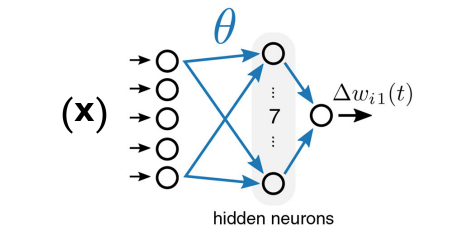
\includegraphics[scale=.5]{metaplasticity.png}
  }}
  \caption{ MLP architecture of meta-plasticity with inputs $\mathbf{(x)}$, one hidden layer of seven neurons and parameters $\theta$. 
  The network outputs the weight updates for the agent-network.
  (edited from \cite{bohnstinglNeuromorphicHardwareLearns2019}).
  }
        \label{figurelabel}
     \end{figure}

The resulting learning rule $f_{ANN}(\mathbf{x_{ji}}(t);\theta)$ is called meta-plasiticity and offers 
a new perspective on how synaptic 
plasticity in SNNs may be adjusted to boost performance on whole task families. Meta-plasticity, polished over various tasks
of a family F, may enable an SNN-based learner to better perform on each of these tasks by adhering to the simple weight update rule (23):

$$
\Delta w_{ji}=f_{ANN}(\mathbf{x_{ji}}(t);\theta) \eqno{(23)}
$$

Bohnstingl et al. conclude, that the algorithm applied in the outer loop of an L2L framework is crucial to 
its function and emphasize the stability offered by CE and ES due the generation of regions of well-working parameters as opposed to single values
in SA. The perspective of declaring even plasticity rules subject to L2L optimization might offer new paths for research and eventually provide
important insights into learning in biological networks of neurons.

\section{APPLICATIONS OF L2L IN ROBOTICS}

Robotics has undergone many successful developments in the recent past with advances being pushed from 
numerous fields of engineering, including that of machine learning. Yet the design process is still a tedious and 
highly taylored one, usually requiring domain expert knowledge. Many of the underlying algorithms in
 control, motion planning and sensoric interpretation require suitable setups of the environment with little room
for variation. For example industrial manipulator robots can perform outstandingly when placed in a fixed production line, yet 
recognizing and grasping everyday objects in a kitchen or workshop poses a much higher challenge, as it requires the skill to 
make sense of broad environments with numerous imaginable tasks. Furthermore the dominating problems of applying RL in 
robotics can be summarized by the following problem classes \cite{rivlinReinforcementLearningRealWorld2019}:

\begin{itemize}
        \item Sample efficiency
        \item Sim2Real
        \item Reward function optimization
        \item Safety
\end{itemize}   

The previous sections revealed a high potential in L2L frameworks in terms of sample efficiency and generalization, thus constituting 
feasible answers to expensive data generation or overfitting to simulator-specific features. However this further implies a 
reflection on the scalability of said L2L approaches in order to evaluate their applicability in the often very
high-dimensional task spaces faced in robotics. \newline
Wang et al.\cite{wangLearningReinforcementLearn2016} examine meta-RL's ability to detect abstract task 
structures in large scale problems by adapting a well-known behavioural experiment 
described by Harlow \cite{harlowFormationLearningSets1949} to a visual fixation task. In Harlows experiment, 
monkeys were presented two unfamiliar objects, with one 
hiding a bowl filled with food and while the other holds an empty bowl. The monkeys were allowed to choose one
 of the objects and received the reward, if present. 
Despite switching the objects for new unkown objects in each episode, upon replaying several trials in 
several episodes of this game, the animals showed
a general understanding of the underlying structure of the problem. After beginning a new episode with new objects, 
the monkeys would, inevitably, take 
one random guess but managed to succeed in the following trials of the episode \cite{botvinickReinforcementLearningFast2019}. \newline

\subsection{Tasks in high-dimensional spaces}

Motion and path planning are fundamental problems in robotics, whether it be within a space of rich visual input, sensory data or
configuration/joint-spaces. Similiar to the problem described by Harlow, the navigational task in the I-maze environment as described by 
Mirowski et al.\cite{mirowskiLearningNavigateComplex2016} and Jaderberg et al.\cite{jaderbergReinforcementLearningUnsupervised2016} 
requires an understanding of the general structure of the problem in order to learn sample-efficiently 
on the specific task. In this case the same maze spawns a goal location on random position within the maze where the agent has to learn
a motion path to the goal in as few trials as possible. The results of Wang et al.\cite{wangLearningReinforcementLearn2016}
 show, that an architecture of stacked LSTM is able to 
solve the task after having conducted one exploration run (finishing the episode in ~100 timesteps) notably faster (~30 timesteps) within few
explotation runs. The reference baseline, a feedforward architecture A3C learner, is not able to solve the problem at all. 
 
\begin{figure}[thpb]
        \centering
        \framebox{\parbox{3in}{
        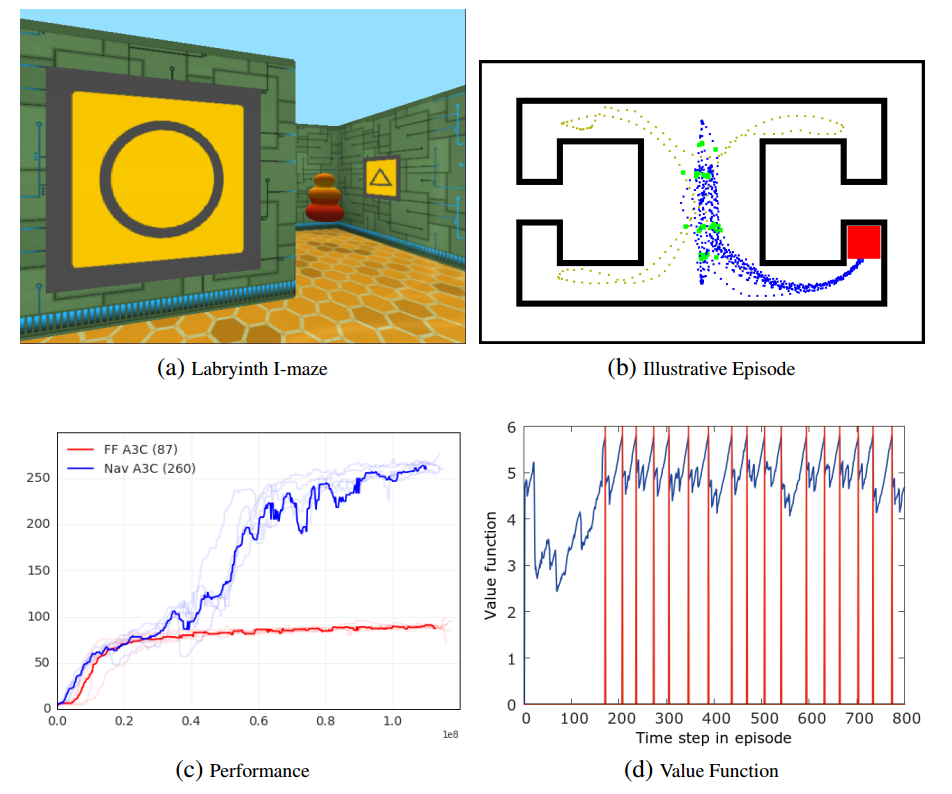
\includegraphics[scale=.2]{Maze_wang.png}
  }}
  \caption{\textbf{a:} I-maze labyrinth view with goal \newline
  \textbf{b:} following initial exploration
  (light trajectories), agent repeatedly goes to goal (blue trajectories). \cite{wangLearningReinforcementLearn2016}
  }
        \label{figurelabel}
     \end{figure}

Duan et al.\cite{duanRLFastReinforcement2016} take a similiar approach in their 
evaluation of the feasbility of RL² in high-dimensional state spaces. Again, a randomly generated 
maze with a randomly placed target is chosen as the problem to solve for the agent. During one test run, the agent is given a number 
of episodes during which the maze structure and target position remain fixed. In contrast to an earlier approach to this RL-Task shown by Oh et al.
\cite{ohZeroShotTaskGeneralization2017} 
RL² bases its actions within a more granular action space. The environments sparse reward payout design (+1 for target, 
-0.001 for wall hits, -0.04 per time frame) poses additional challenges to the agents learning and requires well-devloped exploration strategies 
in the first episode in order to gain information on the problems ground structure. Cross-validation with a small and a larger version of the 
maze environment show a significant reduction in solving trajectory lengths between the first to episodes and indicate, that the RL² algorithm 
managed to utilize previoulsy gained information to come to good solutions more quickly. However the shown results are not yet optimal
as the agent still forgets, though rarely, initially explored target positions and explores further paths in the second episode. Duan et al. 
indicate that further imporvements might come with improved RL-algorithms as the outer-loop optimizer (fig. 15). 

\begin{figure}[thpb]
        \centering
        \framebox{\parbox{3in}{
        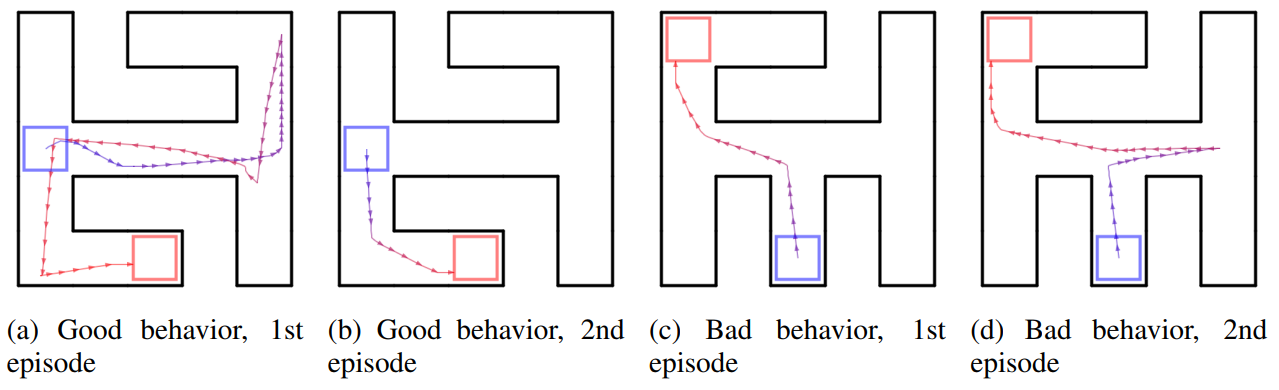
\includegraphics[scale=.17]{duan_maze.png}
  }}
  \caption{Visualization of the agent’s behavior. In each scenario, the agent starts at the center of the
  blue block, and the goal is to reach anywhere in the red block \cite{duanRLFastReinforcement2016}. 
  }
        \label{figurelabel}
     \end{figure}

Bellec et al.\cite{bellecLongShorttermMemory2018} tested an implementation of LSNN on a navigational task in a 
2D arena in reinforcement learning to demonstrate applicability in 
complex environments. The LSNN-based agent was palced in a circular arena in which a specific task $M$ would be to reach a goal within this arena
on a fixed position, while the whole family $F$ of tasks would include various goal positions within this arena. By setting these goal positions 
to be close to the arena boundaries, the agent is challenged to develop an abstract understanding of the commonalities between all tasks, 
which he can exploit when facing one of the tasks $M$. For each of these specific tasks, the objective is 
to reach the goal (at a fixed position throughout one task $M$) as many times as possible within a fixed time frame after being placed randomly
upon reaching the goal. The according sparse reward function was chosen to award goal attainment with a score of 1 while hitting the arena
boundaries will lead to -0.02 punishment. According to the applied L2L framework, outer-loop optimization through BPTT and DEEP-R was performed on the
synaptic weights over the whole task family $F$, while specific task optimization was accomplished by 
adapting the short-term memory, i.e. the thresholds of the adaptive LIF neurons. Remarkably this model was able to generate an abstract understanding
of the characteristic of the task, exhibiting human-like strategies to first explore the boundaries of the given environment to find the goal 
position and utilizing this knowledge to efficiently reach the goal in subsequent runs(fig. 16). 
\begin{figure}[thpb]
        \centering
        \framebox{\parbox{3in}{
        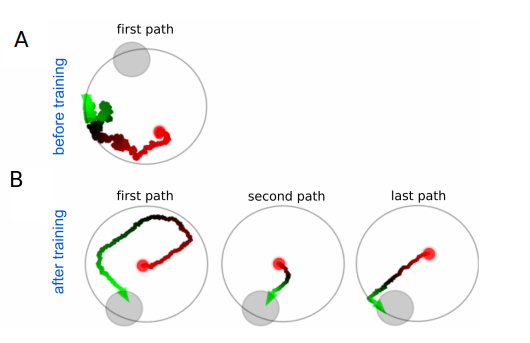
\includegraphics[scale=.4]{lsnn_navigation.png}
}}
\caption{\textbf{A:} The untrained model does not show any strategic or efficient way to find the goal. (Bellec et al.) \newline
\textbf{B:} The trained model performs initial exploration runs alongside environment boundaries, exhibiting the abstract understanding
that all tasks of family $F$ share the characteristic of goals close to the arena boundaries. Efficient path-planning of the agent 
in the subsequent runs prove, that the adaptive LIF neurons were capable of storing the position of the goal in short-term memory. 
\cite{bellecLongShorttermMemory2018}}
        \label{figurelabel}
        \end{figure}
        

\subsection{Few-Shot Learning}

One promising aspect of L2L is the capability of generalizing more than any conventional neural network. A model agile enough to understand
underyling abstract knowledge about robotic motion does not only foreshadow better, more robust motoric control but especially a reduction in 
training data. Bellec et al.\cite{bellecBiologicallyInspiredAlternatives2019} evaluated e-Prop 2 on a one-shot 
learning task, where a trajectory of a 2-joint robotic arm should be learned by 
the agent. That is, the error modules of e-Prop 2 had previously been trained sufficiently on a family of robotic kinematic tasks to generate
fitting learning signals $\hat{L}^t_j$ and RSNN priors $\theta_{init}$. The learning phase of the agent was restricted to a single training run 
to gain a strict evaluation on the capabilities of the L2L system. Interestingly, the agent was not given an inverse kinematic model, thus 
requiring the model to understand the space mismatch between the endeffector pose (network target) in euclidean space and the joint space 
(network output). A family of tasks $F$ was generated with each task $C$ representing a randomly generated target trajectory of the arm endeffector. 
The inner RSNN is a network composed of 400 recurrent LIF neurons which receives inputs $\mathbf{x_t}$ and outputs the required joint velocities 
to influencing the endeffector pose. 
An outer loop error module, consisting of 300 LIF neurons was previously trained with the inputs $\mathbf{x_t}$, spiking activity of the RSNN 
$\mathbf{z^t}$ and the target trajectory $y^{*,t}$ in Euclidean space. The optimization was conducted with BPTT over batches of 
200 different tasks to minimize expectation of the loss sum across the family of tasks. 
\begin{figure}[thpb]
        \centering
        \framebox{\parbox{3in}{
        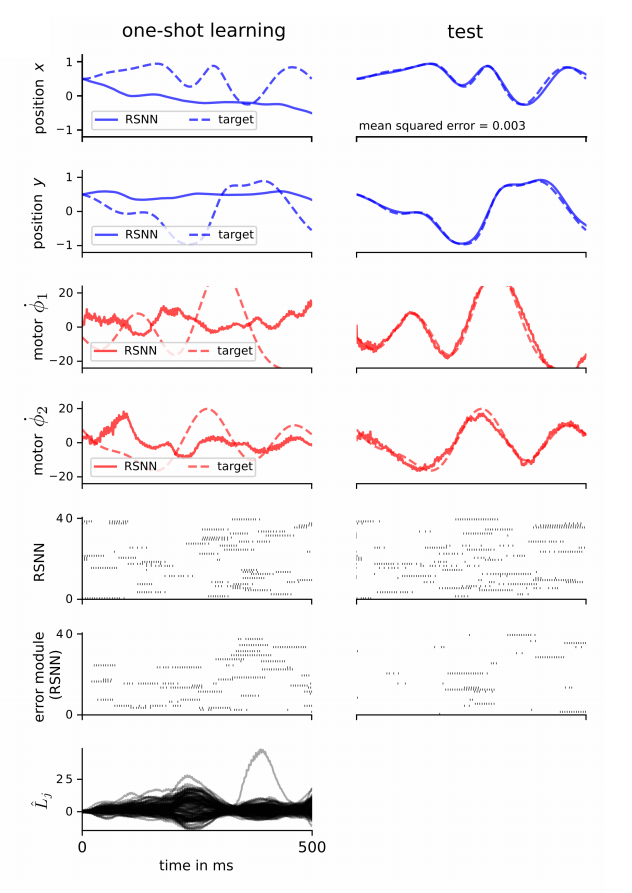
\includegraphics[scale=.35]{eprop2robot.png}
}}
\caption{Results of one-shot learning tasks before (left) and after (right) a single training trial. After a training run, the RSNN 
synpatic weights were updated using learning signal $\hat{L}^t_j$ (bottom). In the fifth row, spikes in the error module have become sparse after
the training run, which can be explained by the low error-rate generated by a learned RSNN \cite{bellecBiologicallyInspiredAlternatives2019}}
        \label{figurelabel}
        \end{figure}

Fig. 17 shows the result of the motor outputs by the RSNN after a single training trial, provided the error modules experienced sufficient training.
In plots 1-4 it becomes apparent, that the first and only training trial was inevitably unsuccesful but generally sufficed to generate trajectories
 with a MSE of 0.003 after a single update of weights with Learning signals from an outer error module. We can 
conclude, that the network has achieved one-shot learning capability for the infinitly large family of random trajectories in a 2-joint robotic arm.

\section{DISCUSSION}
 
The heretofore described framework of L2L and its various applications poses promising persectives for future work in the fields 
of machine learning, robotics but also neuroscience and cognitive sciences. Historically, these fields have been intertwined and underwent
phases of more and phases of less interaction but nonetheless generated implications that could be of scientific use for the other. Cognitive 
sciences provide ideas and inspirations for ever further sophisticated algorithms, while Artificial Neural Networks can offer evaluations of 
plausibility for biological models or in turn stimulate new implications for neuroscience on the basis of well-working algorithmic models. L2L
is particularly intersting when considering the gap in learning efficiency between human brains and ANNs. The idea of certain preshaped 
priors innert to human brains is certainly not new to cognitive sciences and seem quite obvious when taking into account the remarkable 
learning efficiency all humans share. However conclusions on the origin and development of such preengineered priors remain vague
and manifold. Wang et al.\cite{wangPrefrontalCortexMetareinforcement2018} propose,
that midbrain dopamine-driven synaptic plasticity in the brain may well be an outer-loop optimization system shaping 
learning in the prefrontal cortex (PFC), 
which in turn acts as a hierarchically lower learner. The dopamine neurons of the midbrain are thought to employ reward prediction 
error signals which shape synaptic connectivity in such a way that animals are prone to improve performance 
\cite{montagueFrameworkMesencephalicDopamine1996}. Despite this, it is 
up to debate, to which extent these signals contain information which is based on a environment-dependent model (model-based) or occur model-free.
For example, Daw et al.\cite{dawModelbasedInfluencesHumans2011} discovered evidence, that signals strongly correlated to 
dopaminergic prediction errors contain robust model-based
information \cite{botvinickReinforcementLearningFast2019}\cite{dawModelbasedInfluencesHumans2011}.
In this regard, Wang et al.\cite{wangPrefrontalCortexMetareinforcement2018} point out that a meta-RL system trained with a model-free RL algorithm 
can generate model-based like behaviour in the inner loop algorithm. They suggest that very similarly, 
human brains may actually operate in a grey area between 
model-free and model-based RL and do so in coordinance with the uniformity of environmental structures. \newline

Bellec et al.\cite{bellecLongShorttermMemory2018} yield a different interpretation of the nested nature of L2L and argue that 
sophisticated priors and learning algorithms have been
shaped by long evolutionary processes. In fact this perspective alleviates the imminent need for biologically implausible processes such as the 
backpropagation of error-gradient learning signals through multiple layers and even time. By optimizing directly broadcasted learning signals coupled
with eligibility traces of spiking neurons, Bellec et al. were the first to reproduce meta-learning in networks of spiking neurons and provide 
promising results, albeit not yet surpassing the performance of BPTT-based ANNs. \newline

On another note, the implementation and performance of SNNs is strongly linked to the development of fitting neuromorphic hardware and appropriate
algorithms. Taking into consideration the analogy of evolution for L2L, it should come with little surprise that the outer loop optimization of L2L 
is considered a crucial bottleneck in terms of capability and computational efforts \cite{duanBenchmarkingDeepReinforcement}. 
In the light of energy and computation efficiency, 
LSNNs exhibit the remarkable characteristic of sparse firing activity and imply further capabilites in activity-silent memory, much like 
human brains. \newline

Applications of L2L such as the experiments described in previous chapters point at the opportunities of this approach but to this date remain
proof-of-concepts. Duan et al.\cite{duanRLFastReinforcement2016} hold upscaling of L2L for broader distributions of tasks to be 
the most important next step in this approach. It 
is yet to be determined, how L2L models could be combined to generate a single system with dedicated learning modules to tackle applications which 
require vast ranges of skills.
Large-scale projects such as the $Scalable\ Deep\ Reinforcement\ 
Learning\ for\ Robotic\ Manipulation$ by Google Brain\cite{ScalableDeepReinforcement} are evidence of the imminent need for data efficient, 
generalizing learning algorithms, 
especially in the light of the immense efforts currently needed to 
apply deep learning algorithms in robotics. Simulation based projects like $Learning\ Dexterity$ by OpenAI \cite{LearningDexterity2018} 
are challenged by sim2real and 
again invest immense efforts in domain randomization approaches. A network architecture that promises greater generalization ability could hold 
answers for better results in terms of stability and safety as well. Especially when deployed in large machines 
(e.g. industrial robotics, autonomous driving),
Deep Learning is required to adhere to high safety standards with nearly impossible-to-get training data. 
L2L might therefore be part of some of 
the largest upcoming challenges faced in this field.


%\newpage
%\addtolength{\textheight}{-12cm}   % This command serves to balance the column lengths
                                  % on the last page of the document manually. It shortens
                                  % the textheight of the last page by a suitable amount.
                                  % This command does not take effect until the next page
                                  % so it should come on the page before the last. Make
                                  % sure that you do not shorten the textheight too much.

%%%%%%%%%%%%%%%%%%%%%%%%%%%%%%%%%%%%%%%%%%%%%%%%%%%%%%%%%%%%%%%%%%%%%%%%%%%%%%%%



%%%%%%%%%%%%%%%%%%%%%%%%%%%%%%%%%%%%%%%%%%%%%%%%%%%%%%%%%%%%%%%%%%%%%%%%%%%%%%%%



%%%%%%%%%%%%%%%%%%%%%%%%%%%%%%%%%%%%%%%%%%%%%%%%%%%%%%%%%%%%%%%%%%%%%%%%%%%%%%%%

\bibliography{L2L}
\bibliographystyle{plain}



\end{document}
